\documentclass[leqno, openany]{memoir}
\setulmarginsandblock{3.5cm}{3.5cm}{*}
\setlrmarginsandblock{3cm}{3.5cm}{*}
\checkandfixthelayout

\usepackage{amsmath}
\usepackage{amssymb}
\usepackage{amsthm}
%\usepackage{MnSymbol}
\usepackage{bm}
\usepackage{accents}
\usepackage{mathtools}
\usepackage{tikz}
\usetikzlibrary{calc}
\usetikzlibrary{automata,positioning}
\usepackage{tikz-cd}
\usepackage{forest}
\usepackage{braket} 
\usepackage{listings}
\usepackage{mdframed}
\usepackage{verbatim}
\usepackage{physics}
\usepackage{stmaryrd}
\usepackage{mathrsfs} 
\usepackage{ulem} 
\usepackage{stackengine}
%\usepackage{/home/patrickl/homework/macaulay2}

%font
\usepackage[sc]{mathpazo}
\usepackage{eulervm}
\usepackage[scaled=0.86]{berasans}
\usepackage{inconsolata}
\usepackage{microtype}

%CS packages
\usepackage{algorithmicx}
\usepackage{algpseudocode}
\usepackage{algorithm}

% typeset and bib
\usepackage[english]{babel} 
\usepackage[utf8]{inputenc} 
\usepackage[T1]{fontenc}
\usepackage[backend=biber, style=alphabetic]{biblatex}
\usepackage[bookmarks, colorlinks, breaklinks]{hyperref} 
\hypersetup{linkcolor=blue,citecolor=magenta,filecolor=black,urlcolor=blue}
\usepackage{cleveref}

% other formatting packages
\usepackage{float}
\usepackage{booktabs}
\usepackage[shortlabels]{enumitem}
\usepackage{csquotes}
\usepackage{titlesec}
\usepackage{titling}
\usepackage{parskip}
\usepackage{graphicx}
\graphicspath{{./}}

\usepackage{lipsum}

% delimiters
\DeclarePairedDelimiter{\gen}{\langle}{\rangle}
\DeclarePairedDelimiter{\floor}{\lfloor}{\rfloor}
\DeclarePairedDelimiter{\ceil}{\lceil}{\rceil}


\newtheorem{thm}{Theorem}[section]
\newtheorem{cor}[thm]{Corollary}
\newtheorem{prop}[thm]{Proposition}
\newtheorem{lem}[thm]{Lemma}
\newtheorem{conj}[thm]{Conjecture}
\newtheorem{quest}[thm]{Question}

\theoremstyle{definition}
\newtheorem{defn}[thm]{Definition}
\newtheorem{defns}[thm]{Definitions}
\newtheorem{con}[thm]{Construction}
\newtheorem{exm}[thm]{Example}
\newtheorem{exms}[thm]{Examples}
\newtheorem{notn}[thm]{Notation}
\newtheorem{notns}[thm]{Notations}
\newtheorem{addm}[thm]{Addendum}
\newtheorem{exer}[thm]{Exercise}

\theoremstyle{remark}
\newtheorem{rmk}[thm]{Remark}
\newtheorem{rmks}[thm]{Remarks}
\newtheorem{warn}[thm]{Warning}
\newtheorem{sch}[thm]{Scholium}


% unnumbered theorems
\theoremstyle{plain}
\newtheorem*{thm*}{Theorem}
\newtheorem*{prop*}{Proposition}
\newtheorem*{lem*}{Lemma}
\newtheorem*{cor*}{Corollary}
\newtheorem*{conj*}{Conjecture}

% unnumbered definitions
\theoremstyle{definition}
\newtheorem*{defn*}{Definition}
\newtheorem*{exer*}{Exercise}
\newtheorem*{defns*}{Definitions}
\newtheorem*{con*}{Construction}
\newtheorem*{exm*}{Example}
\newtheorem*{exms*}{Examples}
\newtheorem*{notn*}{Notation}
\newtheorem*{notns*}{Notations}
\newtheorem*{addm*}{Addendum}


\theoremstyle{remark}
\newtheorem*{rmk*}{Remark}

% shortcuts
\newcommand{\Ima}{\mathrm{Im}}
\newcommand{\A}{\mathbb{A}}
\newcommand{\F}{\mathbb{F}}
\newcommand{\G}{\mathbb{G}}
\newcommand{\N}{\mathbb{N}}
\newcommand{\R}{\mathbb{R}}
\newcommand{\C}{\mathbb{C}}
\newcommand{\Z}{\mathbb{Z}}
\newcommand{\Q}{\mathbb{Q}}
\renewcommand{\k}{\Bbbk}
\renewcommand{\L}{\mathbb{L}}
\renewcommand{\P}{\mathbb{P}}
\newcommand{\M}{\overline{M}}
\newcommand{\g}{\mathfrak{g}}
\newcommand{\h}{\mathfrak{h}}
\newcommand{\n}{\mathfrak{n}}
\renewcommand{\b}{\mathfrak{b}}
\newcommand{\ep}{\varepsilon}
\newcommand*{\dt}[1]{%
   \accentset{\mbox{\Huge\bfseries .}}{#1}}
\renewcommand{\abstractname}{Official Description}
\newcommand{\mc}[1]{\mathcal{#1}}
\newcommand{\T}{\mathbb{T}}
\newcommand{\mf}[1]{\mathfrak{#1}}
\newcommand{\mr}[1]{\mathrm{#1}}
\newcommand{\ms}[1]{\mathsf{#1}}
\newcommand{\mt}[1]{\mathtt{#1}}
\newcommand{\on}[1]{\operatorname{#1}}
\newcommand{\ol}[1]{\overline{#1}}
\newcommand{\ul}[1]{\underline{#1}}
\newcommand{\wt}[1]{\widetilde{#1}}
\newcommand{\wh}[1]{\widehat{#1}}
\renewcommand{\div}{\operatorname{div}}
\newcommand{\bir}{\sim_{\mr{bir}}}
\newcommand{\stacks}[1]{\href{https://stacks.math.columbia.edu/tag/#1}{#1}}
\newcommand{\ostar}{\stackMath\mathbin{\stackinset{c}{0ex}{c}{0ex}{\star}{\bigcirc}}}

\DeclareMathOperator{\Der}{Der}
\DeclareMathOperator{\Def}{Def}
\DeclareMathOperator{\Bl}{Bl}
\DeclareMathOperator{\NE}{NE}
\DeclareMathOperator{\Tor}{Tor}
\DeclareMathOperator{\Hom}{Hom}
\DeclareMathOperator{\Ext}{Ext}
\DeclareMathOperator{\End}{End}
\DeclareMathOperator{\ad}{ad}
\DeclareMathOperator{\Aut}{Aut}
\DeclareMathOperator{\Rad}{Rad}
\DeclareMathOperator{\Pic}{Pic}
\DeclareMathOperator{\supp}{supp}
\DeclareMathOperator{\Supp}{Supp}
\DeclareMathOperator{\sgn}{sgn}
\DeclareMathOperator{\spec}{Spec}
\DeclareMathOperator{\Spec}{Spec}
\DeclareMathOperator{\proj}{Proj}
\DeclareMathOperator{\Proj}{Proj}
\DeclareMathOperator{\ord}{ord}
\DeclareMathOperator{\Div}{Div}
\DeclareMathOperator{\depth}{depth}
\DeclareMathOperator{\coker}{coker}
\DeclareMathOperator{\ch}{ch}

% Section formatting
\titleformat{\section}
    {\Large\sffamily\scshape\bfseries}{\thesection}{1em}{}
\titleformat{\subsection}[runin]
    {\large\sffamily\bfseries}{\thesubsection}{1em}{}
\titleformat{\subsubsection}[runin]{\normalfont\itshape}{\thesubsubsection}{1em}{}

\title{COURSE TITLE}
\author{Lectures by INSTRUCTOR, Notes by NOTETAKER}
\date{SEMESTER}

\newcommand*{\titleSW}
    {\begingroup% Story of Writing
    \raggedleft
    \vspace*{\baselineskip}
    {\Huge\itshape Integrability, Enumerative Geometry, and Quantization \\ August-September 2022}\\[\baselineskip]
    {\large\itshape Notes by Patrick Lei}\\[0.2\textheight]
    {\Large Lectures by Various}\par
    \vfill
    {\Large \sffamily Simons Center for Geometry and Physics}
    \vspace*{\baselineskip}
\endgroup}
\pagestyle{simple}

\chapterstyle{ell}


%\renewcommand{\cftchapterpagefont}{}
\renewcommand\cftchapterfont{\sffamily}
\renewcommand\cftsectionfont{\scshape}
\renewcommand*{\cftchapterleader}{}
\renewcommand*{\cftsectionleader}{}
\renewcommand*{\cftsubsectionleader}{}
\renewcommand*{\cftchapterformatpnum}[1]{~\textbullet~#1}
\renewcommand*{\cftsectionformatpnum}[1]{~\textbullet~#1}
\renewcommand*{\cftsubsectionformatpnum}[1]{~\textbullet~#1}
\renewcommand{\cftchapterafterpnum}{\cftparfillskip}
\renewcommand{\cftsectionafterpnum}{\cftparfillskip}
\renewcommand{\cftsubsectionafterpnum}{\cftparfillskip}
\setrmarg{3.55em plus 1fil}
\setsecnumdepth{subsection}
\maxsecnumdepth{subsection}
\settocdepth{subsection}

\begin{document}
    
\begin{titlingpage}
\titleSW
\end{titlingpage}

\thispagestyle{empty}
\section*{Disclaimer}%
\label{sec:disclaimer}

These notes were taken during the program using the \texttt{vimtex} package of the editor \texttt{neovim}. 
Any errors are mine and not the speakers'. 
In addition, my notes are picture-free (but will include commutative diagrams) and are a mix of my mathematical style and that of the lecturers. Also, notation may differe between lecturers.
If you find any errors, please contact me at \texttt{plei@math.columbia.edu}.

\section*{Acknowledgements}

I would like to thank Ga\"etan Borot, Alexandr Buryak, Melissa Liu, Nikita Nekrasov, Paul Norbury, and Paolo Rossi for organizing this program.

\vspace*{1cm}

\noindent\textbf{Program Website:}  \url{https://scgp.stonybrook.edu/archives/33309}
\newpage

\tableofcontents

\chapter{Virasoro constraints in enumerative geometry (Alexei Oblomkov)}%
\label{cha:alexei}

Here is an equation of a plane curve over formal power series in $s$, which we will call the \textit{Lambert curve}:
\[ ye^y = xe^x e^{-s}. \]
This curve appears in the work of Oblomkov-Okounkov-Pandharipande which treats the descendent Gromov-Witten/Pandharipande-Thomas correspondence in the stationary, non-fully equivariant case. The main question is to consider deformations of this curve.

We will now state the main formula of interest:
\begin{equation}\label{eqn:maineqn} 
    H^{\mr{GW}}(x) = \frac{x}{\theta} \Res_{w=\infty} \qty(\frac{\sqrt{\dd{y} \dd{w}}}{y-w}; e^{\theta \phi(y) - \theta \phi(w)}). 
\end{equation}
This formula lives on the curve $ye^{y} = we^{w} e^{-x/\theta}$, where $\theta^{-2} = -c_2(T_X)$ for $X$ a compact threefold. Here, we define
\[ \phi(z) = \sum_{n > 0} \frac{a_n}{n} \qty(\frac{izc_1}{u})^{-n} + \frac{1}{c_1} \sum_{n < 0} \frac{a_n}{n} \qty(\frac{izc_1}{u})^{-n}. \]
The $a_n$ satisfy the usual Heisenberg relations $[a_n, a_m] = m \delta_{n+m, 0}$.

\begin{thm}[Oblomkov-Okounkov-Pandharipande]
    There is an equality (after the standard change of variables $q=-e^{iu}$ and up to a monomial in $q$) of equivariant $2$-legged vertices with descendents
    \[ \braket{\prod_{i=1}^m H_{k_i}^{\mr{GW}}(p)}{\mu_1, \mu_2, \emptyset}^{\mr{GW}} = q^? \braket{\prod_{i=1}^m H_{k_i}^{\mr{PT}}(p)}{\mu_1, \mu_2, \emptyset}^{\mr{PT}} \]
    modulo $(s_1+s_2)(s_2+s_3)$, where
    \[ H^{\mr{PT}}(x) = S^{-1} \qty(\frac{x}{\theta}) \sum_{k=0}^{\infty} x^k \ch_k(\F-\mc{O}), \]
    where $\F$ is the universal stable pair on the PT moduli space. Here, we have
    \[ S(z) = \frac{e^{z/2}-e^{-z/2}}{z}. \]
\end{thm}

\section{GW/Hurwitz correspondence for curves}

\subsection{Hurwitz theory}\label{sub:hurwitz}

Hurwitz theory counts ramified covers of a curve $X$ with specified ramification data:
\[ H^X_d(\eta^1, \ldots, \eta^n) = \# \qty{\pi \colon C \to X \mid \pi^{-1}(z_i) = \eta^i}. \]
Hurwitz proved that these numbers are always finite and that
\[ H^{\P^1}_d(\eta^1, \ldots, \eta^m) = \frac{1}{d!} [C_{(1^d)}] \prod C_{\eta^i} = \frac{1}{(d!)^2} \tr_{\Q S(d)} \prod C_{\eta^i}, \]
where $C_{\eta} = \sum_{g \sim (\eta)} g \in \Q S(d)$ is actually in the center of $\Q S(d)$. Then $C_{\eta}$ acts on $L_{\lambda}$ by the constant function $f_{\eta}(\lambda) = \abs{C_{\eta}} \frac{\chi_{\eta}^{\lambda}}{\dim(\lambda)}$. 

Because of this, we can write
\[ \prod C_{\eta^i} = \sum_{\abs{\lambda} = d} \qty(\frac{\dim \lambda}{d!})^2 \prod_{i=1}^n f_{\eta^i}(\lambda). \]
This can now be computed by a hook length formula, which corresponds to localization in the Hilbert scheme of points on $\C^2$. If we fix $\eta$, then the function 
\[ f_{\eta}(\lambda) = f_{\eta}^{\lambda} \in \Q[\lambda_1, \ldots, \lambda_n]^{* S(n)} \]
is a symmetric function on $(\lambda_i - i)$, or a so-called \textit{shifted symmetric function}. If we consider the limit
\[ \Lambda^* = \varprojlim_{n} \Q[\lambda_1, \ldots, \lambda_n]^{*S(n)}, \]
this is a free algebra on functions $f^{(i)}$ satisfying $f^{(i+1)}(\lambda_1, \ldots, \lambda_i, 0) = f^{(i)}(\lambda_1, \ldots, \lambda_n)$. We now consider the functions
\[ \P_k(\lambda) = \sum_{i=1}^{\infty} \qty(\qty[\lambda_i - i + \frac{1}{2}]^k - \qty(-i + \frac{1}{2})^k) + (1-2^{-k}) \zeta(-k). \]
By the work of Vershik-Kerov, the shifted Schur functions can be written as 
\[ f_{\mu} = \frac{1}{\prod_{\mu_i}} \P_{\mu} + \cdots, \]
which after inversion becomes
\[ \frac{\P_{\mu}}{\prod \mu_i} = f_{\mu} + \sum_{\abs{\lambda} < \abs{\mu}} \rho_{\mu, \lambda} f_{\lambda}. \]
We can also write the completed conjugacy classes $\overline{C}_{\mu} = C_{\mu} + \sum \rho_{\mu, \lambda} C_{\lambda}$.

\begin{exm}
    For example, we have $\overline{(4)} = (4) + 2(2,1) + \frac{5}{4} (2)$.
\end{exm}

\subsection{GW/Hurwitz correspondence}

\begin{thm}[Okounkov-Pandharipande, 2001]\label{thm:op01}
    There is a correspondence
    \[ \tau_k(\omega) = \frac{1}{k!} \ol{(k+1)} \]
    between Gromov-Witten descendents and Hurwitz objects, where $\omega \in H^2(X)$ is the class of a point. More precisely, we have
    \[ \ev{\prod_{k=1}^n \tau_{k_i}(\omega)}_d^{\bullet X} = H_d^X \qty(\prod \frac{\ol{(k_i+1)}}{k_i!}). \]
\end{thm}

This can be related to PT theory as follows: consider $Z = \C^2 \times \P^1$ with the antidiagonal action of $\C^{\times}$ on $\C^2$ and recall that $H_{\C^{\times}}^*(\mr{pt}) = \C[t]$. Then we have the localization formula
\[ \ev{\prod_{i=1}^n \tau_{k_i}(\omega)}_d^{\bullet Z, \C^{\times}} = t^? \ev{\prod_{i=1}^n \tau_{k_i}(\omega)}^{\bullet \P^1}. \]
The left hand side becomes
\begin{align*}
    \ev{\prod_{i=1}^n \ch_{k_i+2}(\omega)}^{\bullet Z, \C^{\times}}_d &= \int_{\mr{Hilb}_d(\C^2) \ch_{k_i+2}(\omega)} \\
    &= H^{\P^1} \qty(\prod_{i=1}^n \frac{\ol{(k_i+1)}}{k_i!}),
\end{align*}
where $\tau_k(\omega) = \ch_{k+2}(\omega)$.

\subsection{PT theory}

For a threefold $Z$, Pandharipande-Thomas theory considers moduli spaces
\[ P_n(Z, \beta) = \qty{[\mc{O}_Z \xrightarrow{\varphi} \mc{F}]} \]
of \textit{stable pairs}, where $\mc{F}$ is a pure dimension $1$ sheaf on $X$ supported on $\beta \in H_2(Z)$ and $n = \ell(\mc{F}/\varphi(\mc{O}_Z))$. This has technical advantages over the older Donaldson-Thomas theory, one of them being that we don't have to study the Hilbert scheme of points on $\C^3$. If we let $\mc{O}_{\P_n(Z, \beta) \times Z} \to \F$ be the universal stable pair, then we define
\[ \ch_k(\gamma) = \int_Z \ch_k(\F) \cup \gamma \] for any $\gamma \in H^*(Z)$.

Now consider $Z = \C^2 \times \P^1$. Then the first nonempty PT moduli space is
\[ P_d(Z, d \P^1) = \mr{Hilb}_d(\C^2). \]
If we let $\gamma \in H_{\C^{\times}}(\C^2)$, we define
\[ \ch_k(\gamma) = \int_{\C^2} \ch_k(\mc{O}/I) \cup \gamma, \]
where $\mc{I}$ is the universal ideal sheaf on $\mr{Hilb}_d(\C^2) \times \C^2$.

\subsection{Idea of proof of GW/Hurwitz}

We begin with a correspondence between relative Gromov-Witten theory without descendents and Hurwitz theory. Then we can degenerate our target curve with descendents to bubble out the descendents. We now need to show that
\[ H_d^{\P^1} \qty(\mu, \frac{\ol{(k+1)}}{k!}) = \mr{GW}^{\P^1}(\mu, \tau_k(\omega)), \]
which requires us to study the equivariant Gromov-Witten theory of $\P^1$.

\subsection{Fock space}\label{sub:fock}

We begin by defining the infinite-dimensional space
\[ V = \bigoplus_{k \in \Z + \frac{1}{2}} \C \ul{k}. \]
Then the semi-infinite exterior power $\bigwedge^{\infty/2} V$ has basis $\qty{\vec{v}_S}$, where $S = \qty{S_1 > S_2 > \ldots} \subset \Z + \frac{1}{2}$ such that
\begin{enumerate}[(i)]
    \item The set $S_+ = S \setminus \qty(\Z_{\leq 0} - \frac{1}{2})$ is finite;
    \item The set $S_- = \qty(\Z_{\leq 0} - \frac{1}{2}) \setminus S$ is also finite.
\end{enumerate}
Then we write $\vec{v}_S = s_1 \wedge s_2 \wedge s_3 \wedge \cdots$.

If we rotate the French way of drawing Young diagrams counterclockwise by $\frac{\pi}{4}$, we obtain the Russian way of drawing Young diagrams:
\begin{figure}[H]
    \centering
    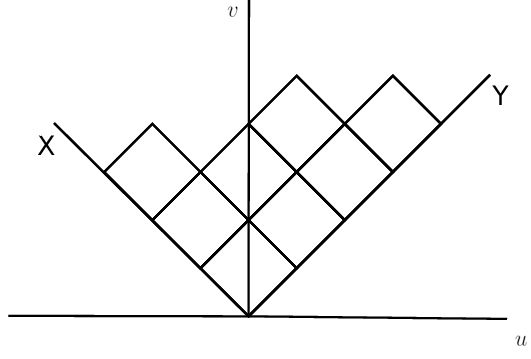
\includegraphics[width=0.6\textwidth]{ydiagru}
    \caption{Russian convention for Young diagrams.}
    \label{fig:ydiagru}
\end{figure}
There are two natural statistics associated to Young diagrams as in \Cref{fig:ydiagru}, which are the size and where the vertex touches the bottom. Define 
\[ V_{\lambda} = \qty(\lambda_1 - \frac{1}{2}) \wedge \qty(\lambda_2 - \frac{3}{2}) \wedge \cdots \]

We now define the operators
\[ \psi_k v = \ul{k} \wedge v. \]
Then we have
\[ :\psi_i \psi_j^*: = \begin{cases}
    \psi_i \psi_j^* & j > 0 \\
    - \psi_j^* \psi_j & j < 0.
\end{cases}
\]
We can check that $[\psi_i, \psi_j] = [\psi_i^*, \psi_j^*] = 0$ and $\psi_i \psi_j^* + \psi_j^* \psi_i = \delta_{ij}$. If we consider $E_{ij} \in \mf{gl}(\infty)$, then assigning $E_{ij} \mapsto \psi_i \psi_j^*$ gives a projective representation of $\mf{gl}(\infty)$. The Casimir operator is $c = \sum_{k \in \Z + \frac{1}{2}} E_{kk}$, and this acts by
\[ c v_S = (\abs{S_+} - \abs{S_-}) v_S. \]
In addition, the operator $H = \sum k E_{kk}$ acts by 
\[ H v_{\lambda} = \abs{\lambda} v_{\lambda}. \]

Define the operators
\[ \mc{E}_r(z) = \sum e^{z(k-r/2)} E_{k-r,k} + \frac{\delta_{r,0}}{\zeta(z)}, \]
where $\zeta(z) = e^{z/2} - e^{-z/2}$. In particular, we have $\mc{E}_r(0) = \sum E_{k-r, k} = \alpha_r$ for $r \neq 0$, where $[\alpha_k, \alpha_r] = k \delta_{k+r}$.

The space $\qty(\bigwedge^{\infty/2} V)_0$ has two natural bases given by the $v_S$ and by $\prod \alpha_{k_i} v_{\emptyset}$, where $v_{\emptyset} = \qty(-\frac{1}{2}) \wedge \qty(-\frac{3}{2}) \wedge \cdots$. The transition function between them is $\chi_{\mu}^{\lambda}$. This appears in the Gromov-Witten theory of $\P^1$:
\begin{align*} 
    \mel**{\mu}{\prod \tau_{k_i}(\omega)}{v}^{\P^1} &= \frac{1}{\zeta(\mu) \zeta(\lambda)} \sum_{\abs{\lambda} = \abs{\mu}} \chi_{\mu}^{\lambda} \chi_{\nu}^{\lambda} \times \prod \frac{\P_{k_i+1}(\lambda)}{(k_i+1)!} \\ 
    &= \mel**{\alpha_{\mu}}{\prod_{i=1}^n \frac{[z^{k_i}] \mc{E}_0(z)}{k_i!}}{\alpha_{\nu}},
\end{align*}
where the last equality uses the formula $[z^k](\mc{E}_0(z)) v_{\lambda} = \P_k(\lambda) v_{\lambda}$. The last formula we will write in this section is the relation
\[ [\mc{E}_a(z), \mc{E}_b(w)] = \zeta\qty(\det \mqty(z & a \\ w & b)) \mc{E}_{a+b}(z+w). \]

\chapter{Counting curves in 1, 3, and 5 dimensions (Andrei Okounkov)}%
\label{cha:andrei}

The main object in Gromov-Witten theory is the moduli space $\mc{M}_{\mr{GW}}$ of stable maps $C \to X$ from a curve to $X$. This is of course highly disconnected, so the genus $g$ component will be weighted by $u^{2g-2}$ while we will hide the degree component for now. One of the major ideas in this subject is to push forward cohomology classes to the moduli of curves, which forms a \textit{cohomological field theory} with rich structure coming from maps between different moduli spaces of curves. Instead, we will push things forward to $X$. Just like we can vary the source curves in families, we can degenerate $X$. Also, automorphisms of $X$ still act on our moduli space.

Our goal is to give a target space space of integrals over $\mc{M}_{\mr{GW}}$. We would like a geometric theory that reproduces the same integrals and an algebraic theory that computes them in some fashion resembling a topological quantum field theory -- for example Chern-Simons theory.

The most basic degeneration of a variety $X$ is to degenerate 
\[ X \rightsquigarrow X_1 \cup_D X_2, \] 
where $D$ is a smooth divisor shared between $X_1$ and $X_2$. If we write $\P = \P(\mc{O}_D \oplus N_{X_i/D})$, we obtain the relation
\[ [X] = [X_1] + [X_2] - [\P] \]
in algebraic cobordism. As proved by Levine-Pandharipande, this relation generates all relations in algebraic cobordism. A similar type of degeneration is the expanded degeneration of Jun Li, which creates an accordion of $\P^1$-bundles.

This fits well into the usual TQFT formalism where the boundary divisor $D = \bigsqcup D_i$ is associated to a vector space $\mc{H}(D) = \bigotimes \mc{H}(D_i)$ and the manifold $X$ is a vector in this space. Because $\mc{H}(D)$ is usually the cohomology of some nice space, it has a product $\cup$, integration, and a form
\[ (\alpha, \beta) = \int \alpha \cup \beta. \]
We can impose conditions at $D$ by either pulling back cohomology classes from $D$ or pushing forward to a cohomology class in $\mc{H}(D)$.

In reality, we have more general degenerations, where we have a degeneration
\[ X \rightsquigarrow \bigcup_i X_i, \]
where the $X_i$ are glued along a simple normal crossings divisor. This has been extensively studied in geometry, for example in logarithmic Gromov-Witten theory, logarithmic Donaldson-Thomas theory of Maulik-Ranganathan, and Brett Parker's ``exploded manifolds.''

\section{Counting curves in 1 dimension}

Now, we will take $\dim X = 1$, so we are studying maps $f \colon C \to X$ from a curve. We can take $X = \P^1$ or even $X = \C$ with the action of $\C^{\times}$. Before we begin, we would like to discuss why we prefer $\dim X$ to be odd. If we consider $X \times \C$, then
\[ [\mc{M}_{\mr{GW}}(X \times \C)]^{\mr{vir}} = [\mc{M}_{\mr{GW}}(X)]^{\mr{vir}} \cup \mr{Eu}(H^1(C, \mc{O}_C) \otimes \C) \ep^{-1}, \] 
where $\ep \in H^2([\mr{pt}/\C^{\times}])$ is a coordinate on $\on{\ms{Lie}} \C^{\times}$. This can be removed by taking $\ep \to \infty$, but doing so is very hard and introduces new problems. However, Mumford tells us
\[ \mr{Eu}(\ep) \otimes \mr{Eu}(-\ep) = (-1)^g \ep^{2g}, \]
and thus changing dimension by $2$ is very easy.

In the case of $\dim X = 1$, the geometric target space theory is just Hurwitz theory, which as in~\Cref{sub:hurwitz} counts ramified covers of $X$ of degree $d$ with specified ramification data. This ramification data is an instance of a relative condition in Gromov-Witten theory, which is as follows. We can consider the moduli space of relative stable maps $\mc{M}_{\mr{GW}}(X/D)$, where we impose that $f^{-1}(D) = \sum \mu_i p_i$, where $\mu$ is a partition and the $p_i$ are the marked points of $C$.

Hurwitz theory has moduli spaces parameterizing maps $C \to X$ which are ramified covers with the specified ramification, where $(X, x_1, \ldots, x_n)$ can vary in moduli. These moduli spaces are finite over the moduli of curves, so the most interesting number is simply the degree of this map, which is the Hurwitz number. Under degenerations $X \rightsquigarrow X_1 \cup X_2$, then the ramification at the node $x_0$ should match. These are called admissible covers; see Harris-Morrison for a reference. This gives us the relation
\[ \mr{Hur}(X, \mu_1, \mu_2, \ldots) = \mr{Hur}(X_1, \mu_1, \ldots, \bullet) \cdot \mr{Hur}(X_2, \mu_2, \ldots, \bullet), \]
where $\bullet = \sum_{\eta} \zeta(\eta) \eta \otimes \eta \in \mc{H} \otimes \mc{H}$. This insertion is inverse to the the pairing on $\mc{H}$.

The general answer for Hurwitz numbers was known to Frobenius and Burnside as
\[ \mr{Hur}(\mu^{(1)}, \mu^{(2)}, \ldots)_X = \sum_{\lambda \in \mr{Irr}(S(d))} \qty(\frac{\dim \lambda}{\abs{S(d)}})^{2-2g} \prod_i (\text{central character of }\mu^{(i)}\text{ in }\lambda). \]
This contains a blueprint for the modern understanding of all 2d TQFTs as well as handle-gluing operators.

\subsection{More algebraic way to think about characters of $S(d)$}

There is the action of a central extension of $\mf{gl}(\infty)$ on $\bigwedge^{\infty/2} \C^{\infty}$, known as the \textit{Fock space}. We need the operators $\psi_k, \psi_k^*$ defined in \Cref{sub:fock}, but we also want the Heisenberg operators
\[ \alpha_n = \sum_{j-i=n} E_{ij}, \]
which act on the vacuum $v_{\emptyset}$ by
\[ \prod \alpha_{-\mu_i} \ket{v_{\emptyset}} = \sum_{\lambda} \chi_{\mu}^{\lambda} \ket{\lambda}. \]

We also want co consider the fermionic operators
\[ P_m = \sum_k k^m \psi_k \psi_k^* \]
taken without the normal ordering and $\zeta$-regularized as in
\[ \sum_{i=1}^{\infty} \qty(-i + \frac{1}{2})^m = (1-2^{-m})\zeta(-m). \]
The operator $P_m$ acts with eigenvalue
\[ p_m(\lambda) = \sum_i \qty(\lambda_i - i + \frac{1}{2})^m \]
on $\ket{\lambda}$. By Vershik-Kerov and Kerov-Olshanski, the central character of $\mu$ and $\lambda$ are polynomials of $\lambda$, which are $\C[p_1, p_2, \ldots]$ and in fact is equal to
\[ \frac{1}{\prod \mu_i} \prod p_{\mu_i} + \cdots, \]
where the lower order terms are controlled by the Gromov-Witten/Hurwitz correspondence. In particular, there is the remarkable formula
\[ \sum z^{d-\frac{1}{24}} \mr{Hur}(\P^1, \mu_1, \ldots) = \mel**{v_{\emptyset}}{e^{\alpha_1} z^{p_1} (\text{fermionic operators}) e^{\alpha_{-1}}}{v_{\emptyset}}, \]
while the case of the elliptic curve is simply the trace of the middle operator without the $e^{\alpha_1}$ terms.

\subsection{Gromov-Witten/Hurwitz correspondence}

There are several features of this correspondence:
\begin{enumerate}
    \item There are no descendents of $1 \in H^0(X, \Q)$ or $H^1(X, \Q)$ in Hurwitz theory. In Gromov-Witten theory, these can be explicitly reduced to descendents of $\mr{pt} \in H^2(X, \Q)$.
    \item Relative conditions correspond to relative conditions. This will always be true in the things that we study.
    \item Descendents of $\mr{pt} \in H^2(X, \Q)$ are equal to relative conditions glued on a $\P^1$ bubble.
\end{enumerate}
This reduces to computing everything in the Gromov-Witten theory of $X = (\P^1, 0, \infty)$, where one of the marked points is descendent and the other is relative.

The remarkable formula in~\Cref{thm:op01} can be computed explicitly and gives a formula for the completed cycles as conjugacy classes. More generally, if we have two relative points, the invariants can be computed explicitly and are B/C-symmetric in $\eta \cup \eta'$. In particular, for $d = 0$, we have
\[ \tau_k(\mr{pt}) v_{\emptyset} = \frac{1}{(k+1)!}(1-2^{-k-1}) \zeta(-k-1), \]
and this was computed by Faber and Pandharipande.

We now want to consider the equivariant theory for $\P^1$.
\begin{thm}[Okounkov-Pandharipande, 2002]
    We have the identity
    \[ \braket{\exp\qty(\sum_{i \geq 0} t_i \tau_i([0]))}{\mu} = \braket{\exp\qty(\sum_{n \geq 1} \wt{t}_n \alpha_n) \wt{W}}{\mu}, \]
    where we take a linear change of times determined by
    \[ \sum_{k \geq 0} x^{k+1} \tau_k([0]) \rightsquigarrow \sum_{n \geq 1} \frac{u^{n-1}x^n}{(1+\ep x) \cdots (n+\ep x)} \alpha_n. \]
\end{thm}

\subsection{Role of integrable systems}

This last formula was found by Getzler and is problematic in the $\ep \to \infty$ limit. Morally, the Gromov-Witten descendents give a quantum integrable system that looks like a free boson or free fermion. By the Kyoto school of integrable systems, there is a classical integrable system for generating functions. In particular, for $\P^1$ with two marked points, the degeneration gives us
\[ \ev{\exp \qty(\sum_{n \geq 1} \wt{t}_n \alpha_n) g \exp\qty(\sum_{n \geq 1} \wt{s}_n \alpha_{-n})}, \]
which is a tau function for the 2-Toda hierarchy and in particular gives a KP hierarchy for linear Hodge integrals in degree $0$.

\begin{rmk}
    These equations differ from the equations found in 2008 by Kazarian, and this is not well-understood.
\end{rmk}

Fundamentally, these equations come from Pl\"ucker relations for $GL(\infty) \hookrightarrow \End(\mr{Fock})$. This is because in $\mr{Fock} \otimes \mr{Fock}$ there is an invariant operator $\sum \psi_k \otimes \psi_k^*$ commuting with $GL(\infty)$. Our goal now is to understand the deformation of the following for $\dim X = 3$:
\begin{enumerate}
    \item The group $GL(\infty)$;
    \item The representation $GL(\infty) \to \End(\mr{Fock})$;
    \item The quantum integrable system;
    \item The invariant operator in $\mr{Fock} \otimes \mr{Fock}$.
\end{enumerate}

\end{document}
